\begin{figure}[H]
	\center{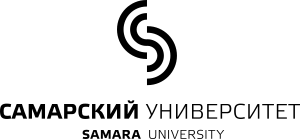
\includegraphics[scale=0.5]{ssau_logo.png}}
\end{figure}
\begin{center}
\tiny{\textbf{МИНОБРНАУКИ РОССИИ\\
ФЕДЕРАЛЬНОЕ ГОСУДАРСТВЕННОЕ АВТОНОМНОЕ\\
ОБРАЗОВАТЕЛЬНОЕ УЧРЕЖДЕНИЕ ВЫСШЕГО ОБРАЗОВАНИЯ\\
<<CАМАРСКИЙ НАЦИОНАЛЬНЫЙ ИССЛЕДОВАТЕЛЬСКИЙ УНИВЕРСИТЕТ\\
ИМЕНИ АКАДЕМИКА С. П. КОРОЛЕВА>>\\}}
\end{center}
\begin{center}
  {Кафедра теоретической механики}
\end{center}
 \vspace{1.5em}
\begin{minipage}{0.5\linewidth}
  \begin{flushleft}
    \end{flushleft}
  \end{minipage}
  \begin{minipage}{0.5\linewidth}
  \begin{flushright}
  УТВЕРЖДАЮ\\
  Заведующий кафедрой\\
  \underline{\hspace{7em}}/Асланов В.С.\\
  <<\underline{\hspace{2em}}>> \underline{\hspace{7em}} 2017 г.\\
  \end{flushright}
 \end{minipage}
  \vspace{0.5em}
  
  \begin{center}
  	\textbf{Задание на выпускную квалификационную работу (ВКР)}
  \end{center}
  
  Студенту \uline{\hfill Асланову Евгению Владмировичу \hfill}группы \uline{1225М}
  \begin{enumerate}
  \item Тема работы \uline{Удаление космического мусора путем электростатического\hfill \break взаимодействия\hfill\break} утверждена приказом по университету от <<\uline{\hspace{2em}}>> \underline{\hspace{7em}} 2017 г. №\underline{\hspace{3em}}
  \item Исходные данные к работе: \uline{параметры пассивного и активного аппаратов:\hfill \break $\phi = 20000$В, $R_1 = 0.5$м, $R_{2a} = R_{2c} = 0.59$м, $R_{2b} = 0.65$м, $l = 1.5$м, $d = 15$м,\hfill \break $J = 1000$кг$\cdot$м${}^2$ \hfill ${}$}
  \item Перечень вопросов, подлежащих разработке в ВКР:
  \uline{1. Метод многих сфер для описания электростатического взаимодействия двух тел. 2.Моделирование\hfill \breakдвижения космического аппарата цилиндрической формы вокруг центра масс при электростатическом взаимодействии с активным спутником при постоянном расстоянии между их центрами масс с помощью метода многих сфер.\hfill \break3. Моделирование движения двух космических аппаратов как двух материальных точек при действии тяги на одном из них. 4. Моделирование движения пассивного космического аппарата цилиндрической формы с активным космическим\hfill \breakаппаратом.\hfill${}$}
  \item Дата выдачи задания: <<\underline{\hspace{2em}}>> \underline{\hspace{7em}} 2017 г.
  \item Срок предоставления на кафедру законченной ВКР: <<\underline{\hspace{2em}}>> \underline{\hspace{6em}} 2017 г.
  \end{enumerate}
\newpage
\noindentРуководитель ВКР\\
$\underset{\text{должность, степень}}{\text{\uline{Заведующий кафедрой, доктор технических наук}}}$
$\underset{\text{подпись}}{\text{\uline{\hspace{10em}}}}$
$\underset{\text{И.О.Фамилия}}{\text{\uline{/В.С. Асланов/}}}$\\
Задание принял к исполнению
$\underset{\text{подпись студента}}{\text{\uline{\hspace{17em}}}}$
$\underset{\text{И.О.Фамилия студента}}{\text{\uline{/\hspace{1em}Е.В. Асланов\hspace{1em}/}}}$